\begin{figure}[htb]
	\centering
	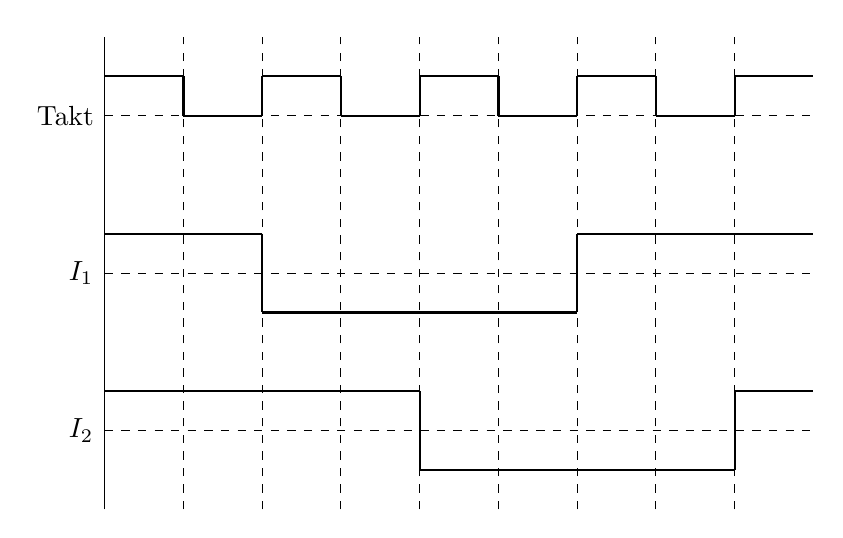
\begin{tikzpicture}
	
	% horizontal axis
	\draw[dashed] (0, 1) -- (9,1);
	\draw[dashed] (0, 3) -- (9,3);
	\draw[dashed] (0, 5) -- (9,5);

	% vertical axis
	\draw (0,0) -- (0,6) node[anchor=east] {};
	\draw[dashed] (1, 0) -- (1,6);
	\draw[dashed] (2, 0) -- (2,6);
	\draw[dashed] (3, 0) -- (3,6);
	\draw[dashed] (4, 0) -- (4,6);
	\draw[dashed] (5, 0) -- (5,6);
	\draw[dashed] (6, 0) -- (6,6);
	\draw[dashed] (7, 0) -- (7,6);
	\draw[dashed] (8, 0) -- (8,6);

	% labels	
	\draw (-0.5, 5) node{Takt};
	\draw (-0.3, 3) node{{$I_1$}};
	\draw (-0.3, 1) node{{$I_2$}};

	%draw Takt
	\draw [thick] (0, 5.5) -- (1, 5.5)
	(1, 5.5) -- (1, 5)
	(1, 5) -- (2, 5)
	(2, 5) -- (2, 5.5)
	(2, 5.5) -- (3, 5.5)
	(3, 5.5) -- (3, 5)
	(3, 5) -- (4, 5)
	(4, 5) -- (4, 5.5)
	(4, 5.5) -- (5, 5.5)
	(5, 5.5) -- (5, 5)
	(5, 5) -- (6, 5)
	(6, 5) -- (6, 5.5)
	(6, 5.5) -- (7, 5.5)
	(7, 5.5) -- (7, 5)
	(7, 5) -- (8, 5)
	(8, 5) -- (8, 5.5)
	(8, 5.5) -- (9, 5.5);
	
	%draw I1
	\draw [thick] (0, 3.5) -- (2, 3.5)
	(2, 3.5) -- (2, 2.5)
	(2, 2.5) -- (6, 2.5)
	(6, 2.5) -- (6, 3.5)
	(6, 3.5) -- (9, 3.5);
	
	%draw I2
	\draw [thick] (0, 1.5) -- (4, 1.5)
	(4, 1.5) -- (4, 0.5)
	(4, 0.5) -- (8, 0.5)
	(8, 0.5) -- (8, 1.5)
	(8, 1.5) -- (9, 1.5);
	
	\end{tikzpicture}
	\caption{Stromverlauf Vollschrittbetrieb Rechtslauf}
	\label{dia:aufg1b_strom}
\end{figure}
